
\chapter{Aufgabe D3}

\section{Simulink-Modell}
Die nachfolgenden Abbildungen zeigen das Simulink-Modell zur Berechnung der Distanzen der einzelnen Räder.\\
Das Modell in \autoref{fig:drivingdistances1} hat die vier Geschwindigkeiten (in km/h) der Räder als Eingänge. Diese werden mit dem \glqq From Workspace"' Block mit ihrer zugehöhrigen Referenzzeit tv in das Model importiert.\\
Danach werden sie in m/s umgerechnet und integriert, um die Strecke zu erhalten. \\
Zur Simulation wird ein FixedStep von 0.01 mit dem ode3-Solver verwendet. Der ode-Solver wurde durch die SImulink \glqq automatic solver selection"' ausgewählt.
\begin{figure}[h!]
	\centering
	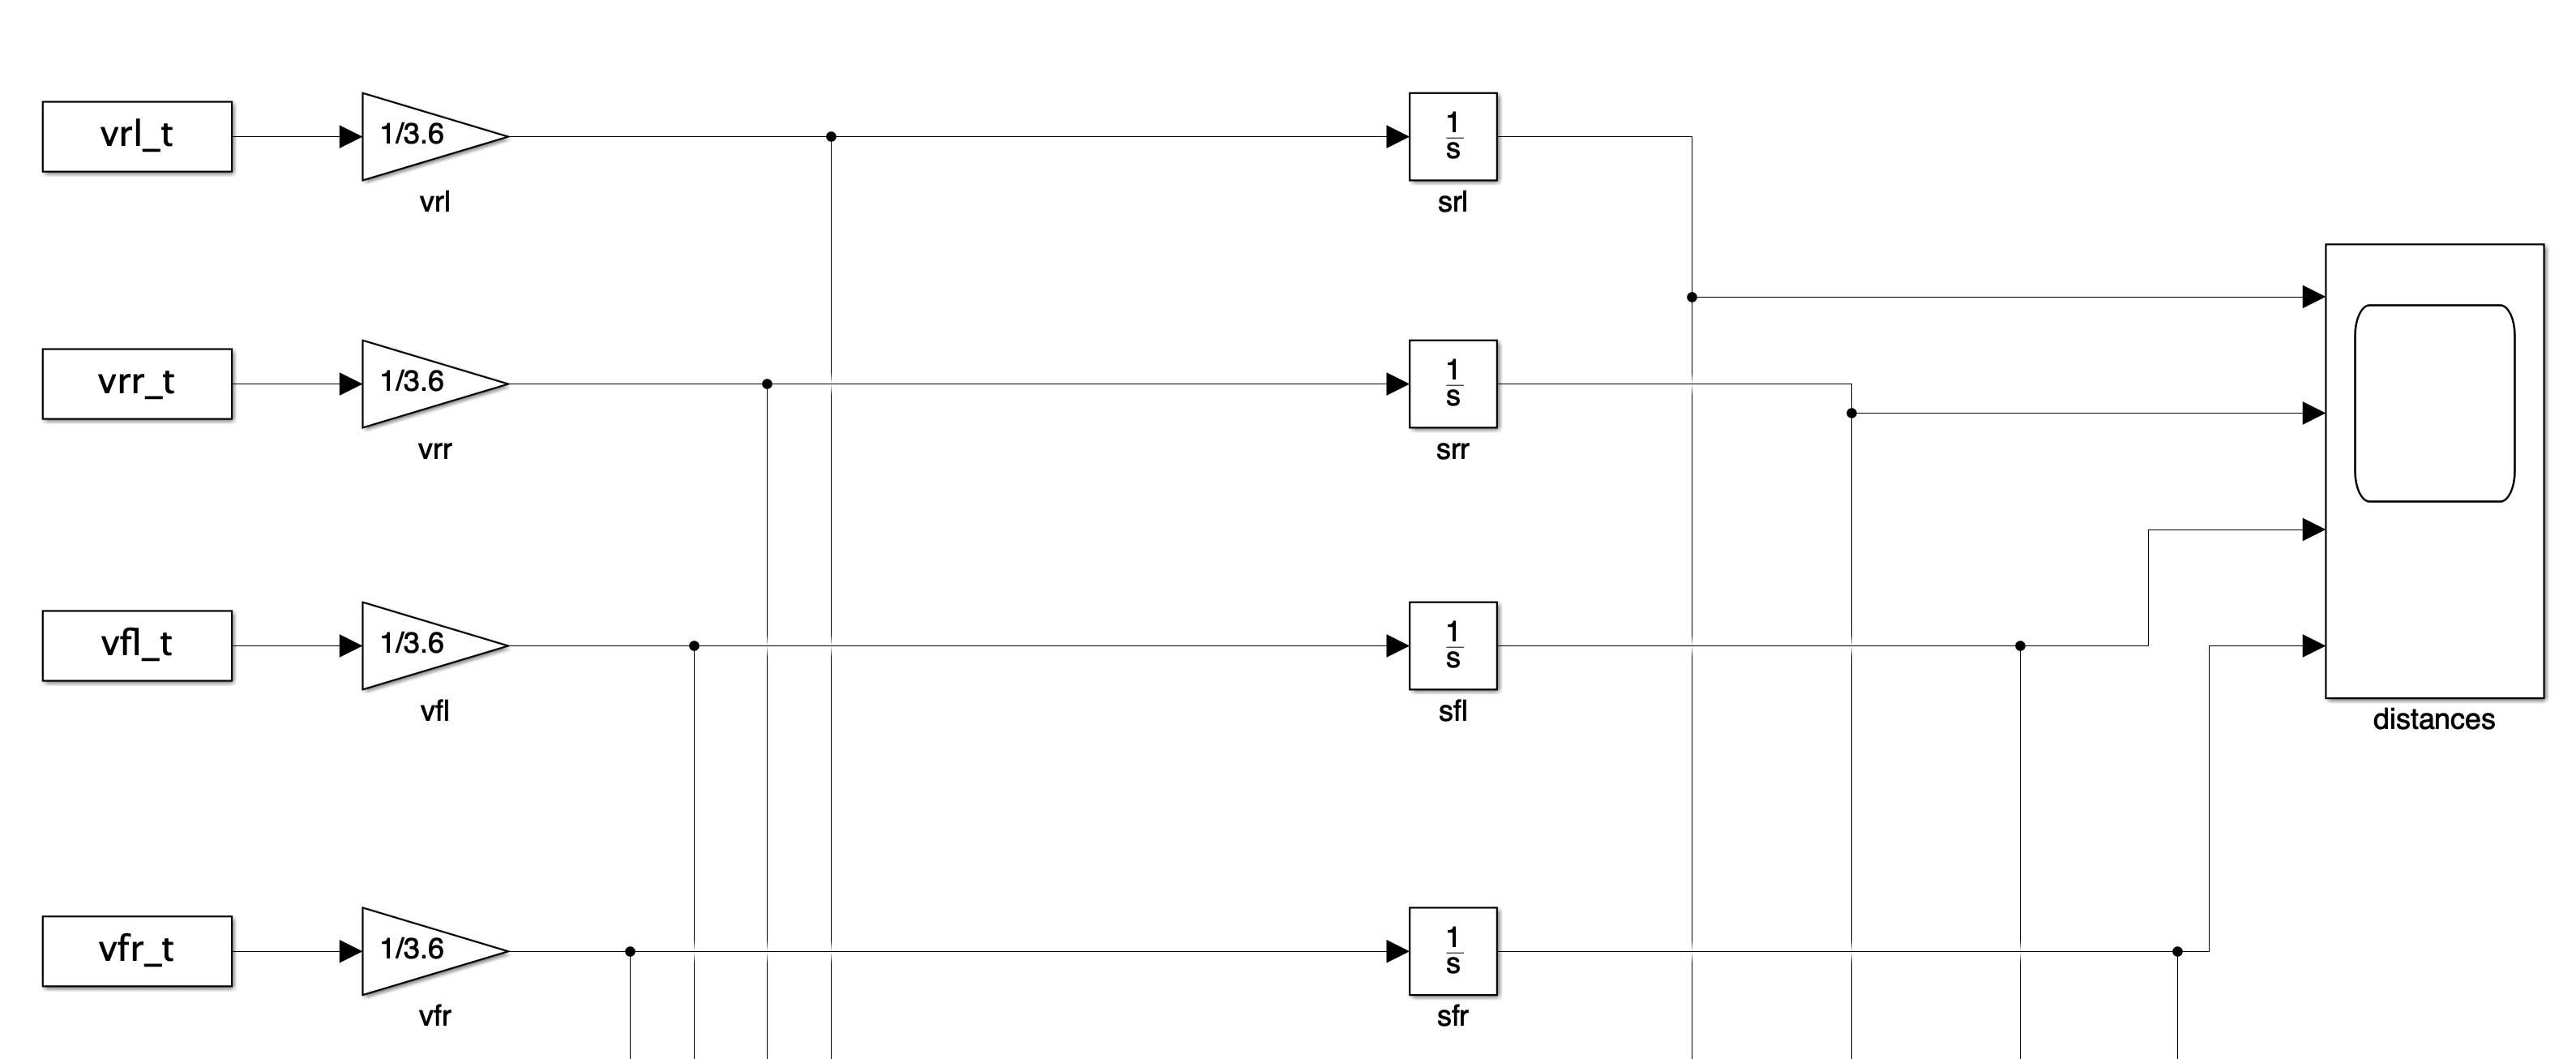
\includegraphics[width=1\linewidth]{../Graphiken/DrivingDistances1}
	\caption{Tire Driving distances}
	\label{fig:drivingdistances1}
\end{figure}
Das Ergebnis der Integration sind die Distanzen der einzelnen Reifen, die gegenüber der Zeit aufgetragen sind.\newpage
\begin{figure}[h!]
	\centering
	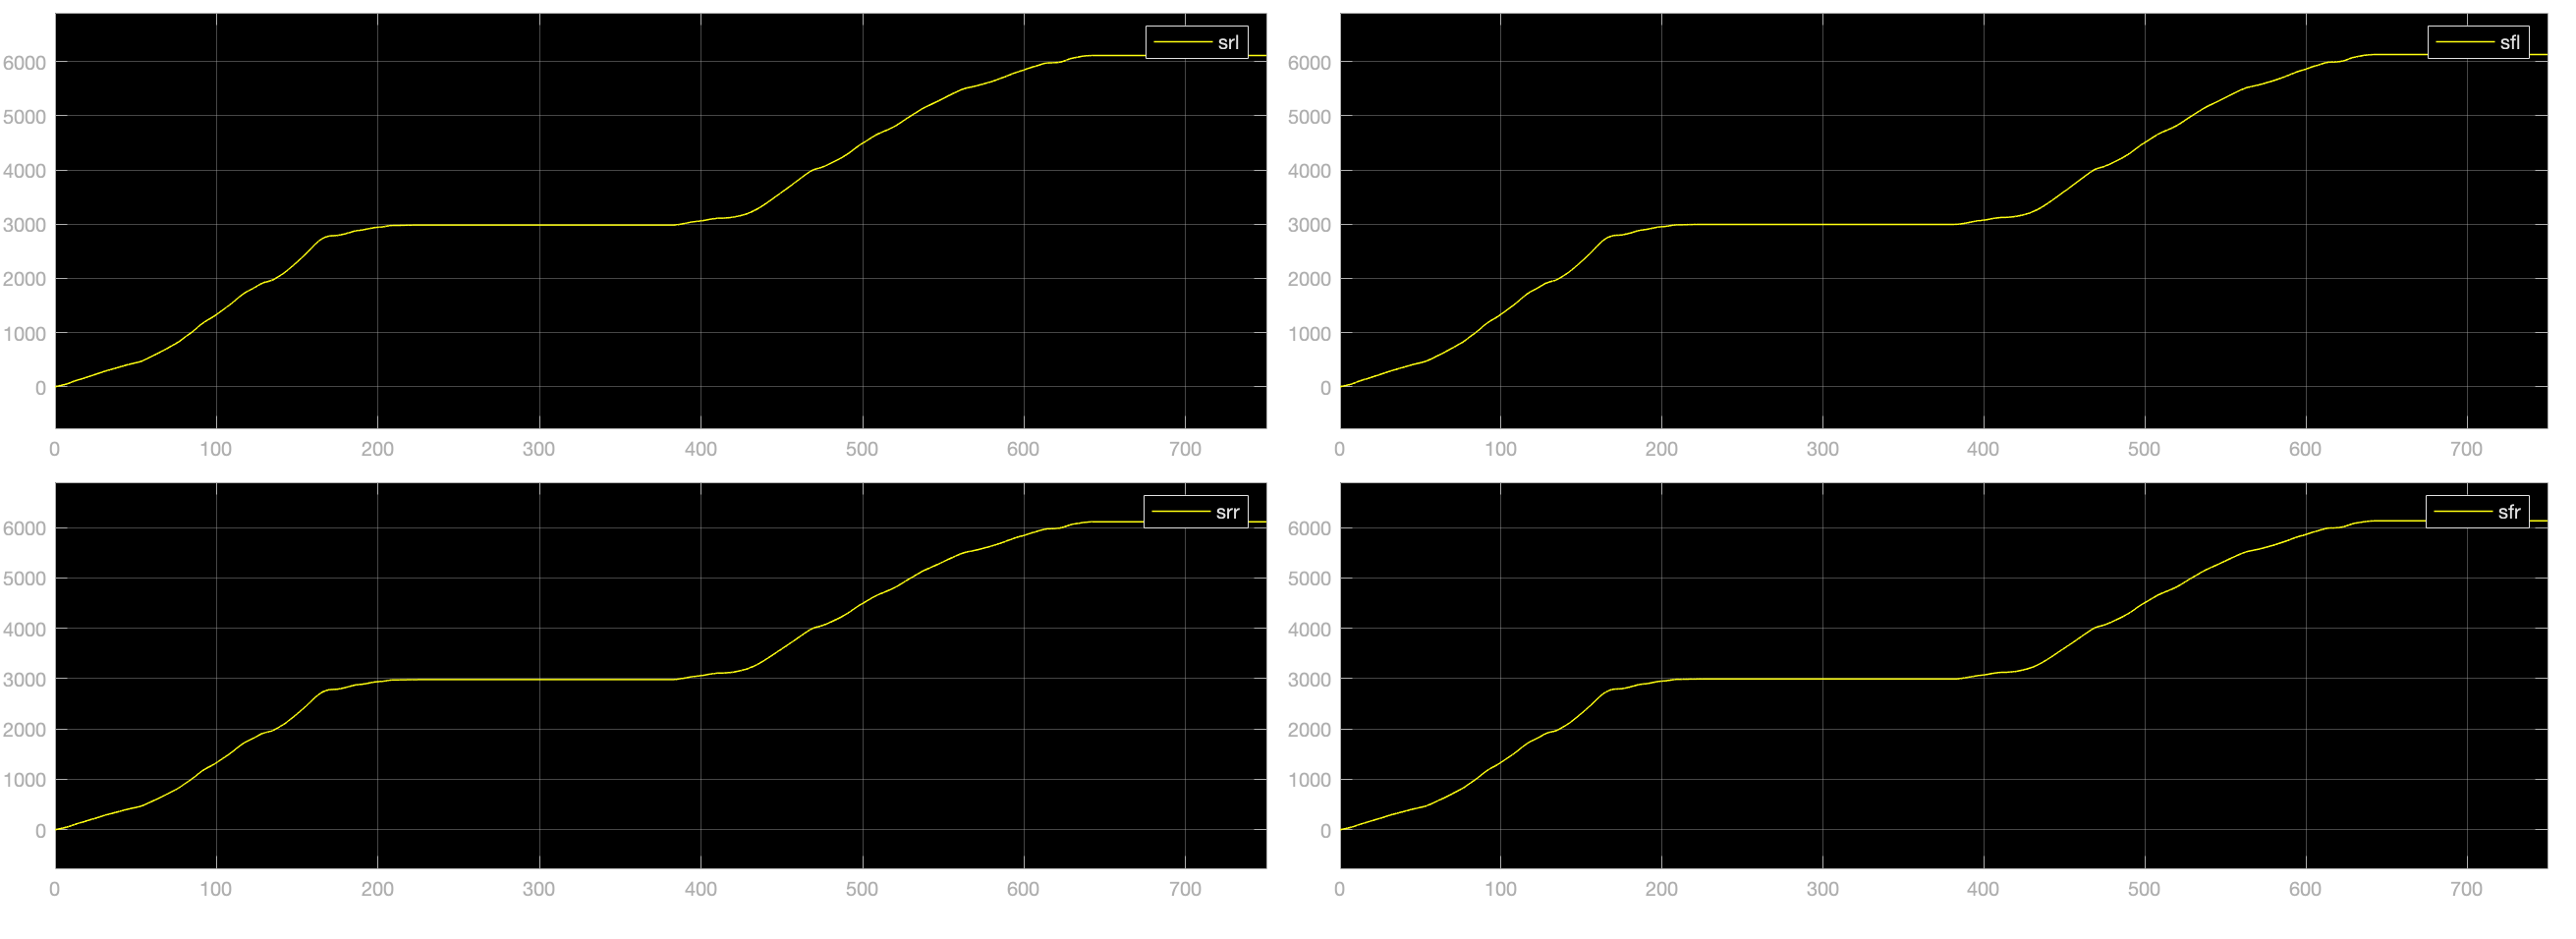
\includegraphics[width=1\linewidth]{../Graphiken/DrivingDistances}
	\caption{Tire Driving distances plot}
	\label{fig:drivingdistances}
\end{figure}

Zur Überprüfung ob es Imbalancen in den Daten gibt wird das Modell wie in \autoref{fig:TireSImCurves} zu sehen ist erweitert.
Der Mittelwert der vier integrierten Distanzen gilt als Referenzwert, ob ein Reifendruckabfall vorliegt. Die Berechnung ist ebenfalls im erweiterten Modell \autoref{fig:TireSImCurves} zusehen. Anschließend wird die prozentuale Abweichung vom Einzelsignal zum Mittelwert berechnet, weicht die Abweichung um mehr als 0.5\% ab handelt es sich um einen Reifendruckabfall. Die Berechnung ist in \autoref{fig:abweichung} dargestellt. \\
\begin{figure}[h!]
	\centering
	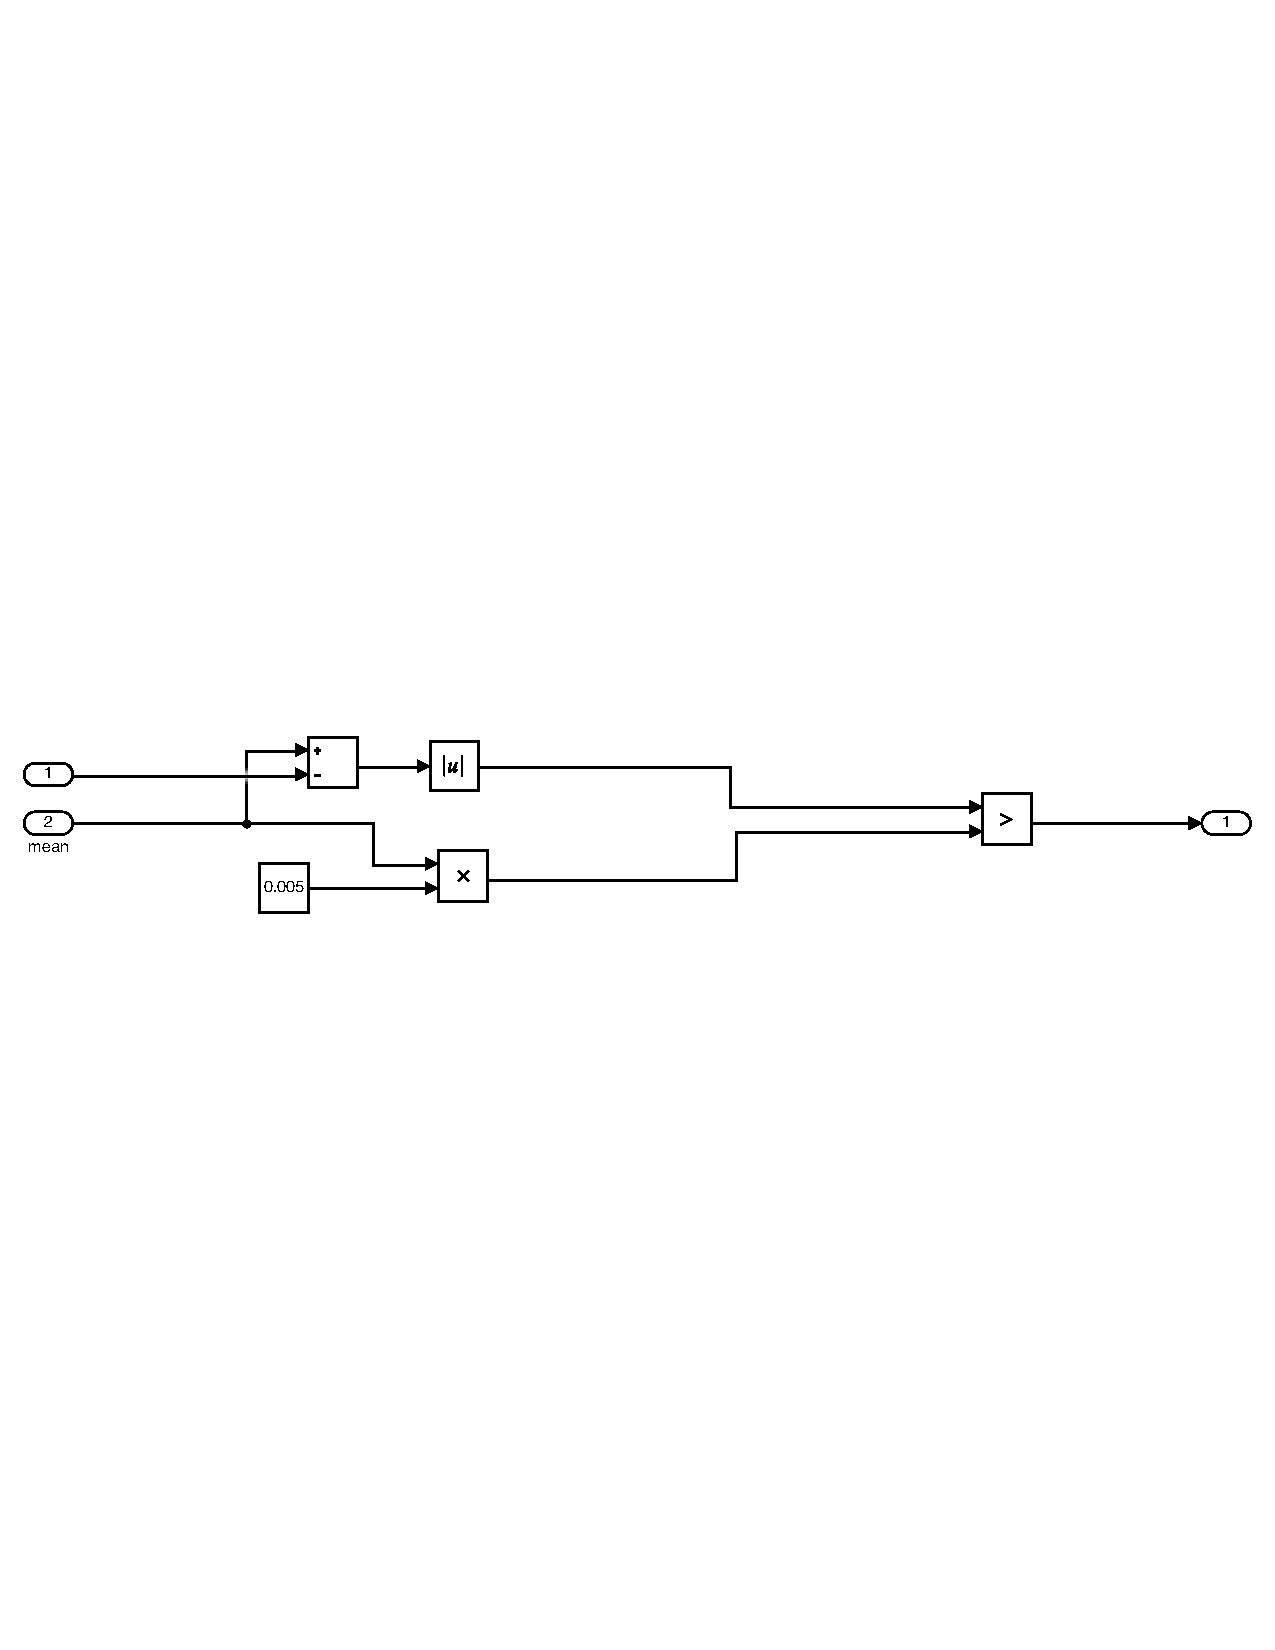
\includegraphics[width=1\linewidth]{../Graphiken/PDFSplit/3_PDFsam_SebastianTireSim2.pdf}
	\caption{Prozentuale Abweichung nach R2}
	\label{fig:abweichung}
\end{figure}
Zur Berechnung wird jedoch nicht das original integrierte Signal der einzelnen Geschwindigkeiten verwendet, sondern die Differenz des integrierten Geschwindigkeitssignals mit dem gleichen Signal um 10 Sekunden nach rechts verschoben. Dadurch werden zur Betrachtung, ob eine Abweichung vorliegt immer nur 10 Sekunden Deltas verwendet. Diese Verschiebung wird mittels des, in \autoref{fig:TireSImCurves} verwendeten, \glqq Transport Delay"' mit einem festen Delay von 10 Zeiteinheiten erzeugt. Danach wird das verspätete Signal von Originalsignal abgezogen um die Deltas zu erhalten.\\
Die Berechnungen für die Abweichungen werden für jeden Reifen einzeln berechnet und anschließend, wie in \autoref{fig:TireSImCurves} zu sehen, verodert, um ein Überblick über das Gesamtsystem zu erhalten.\\

\begin{figure}[H]
	\centering
	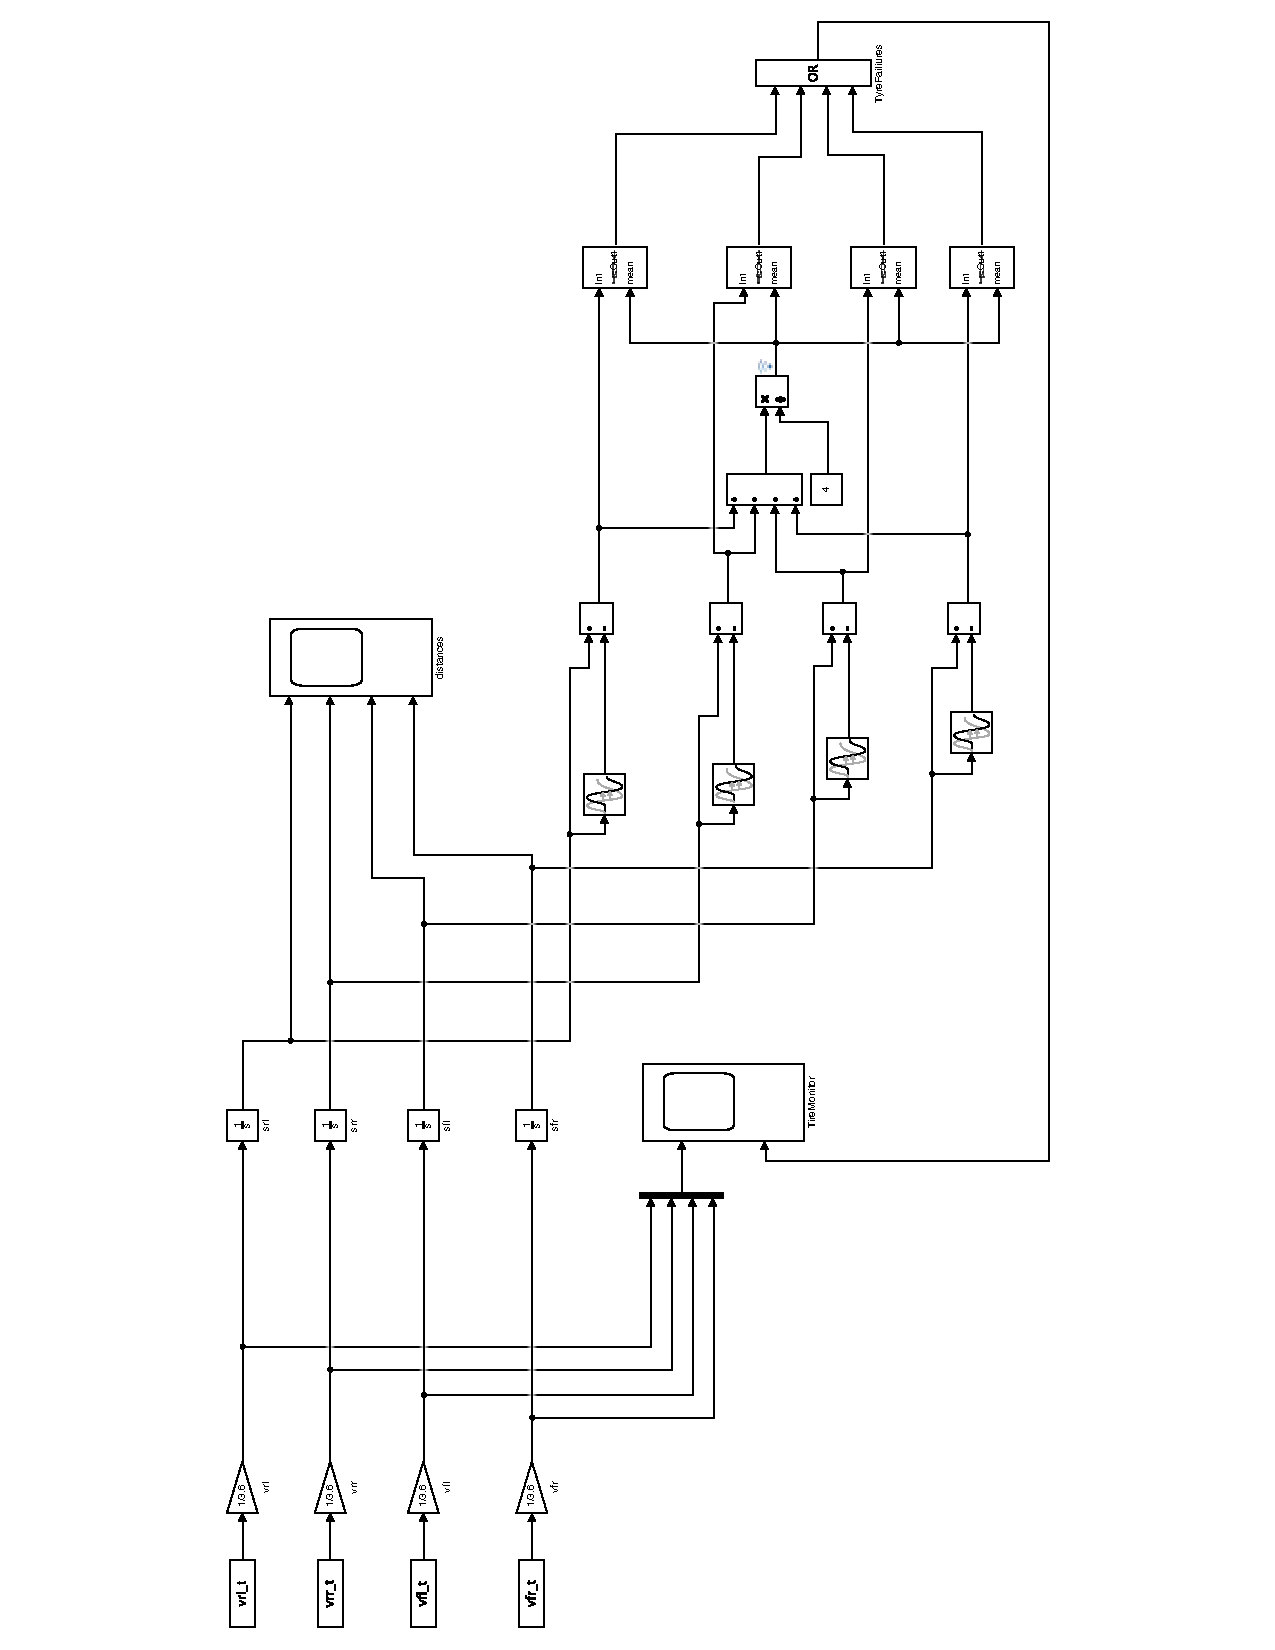
\includegraphics[height=0.95\textheight]{../Graphiken/TireSimCurvesLandscape.pdf}
	\caption{Simulink Tire Distance Model with Curves Data}
	\label{fig:TireSImCurves}
\end{figure}


Für die Kurvenfahrt entsteht die folgende Datenaufzeichnung über die Reifendruckabweichungen.
\begin{figure}[H]
	\centering
	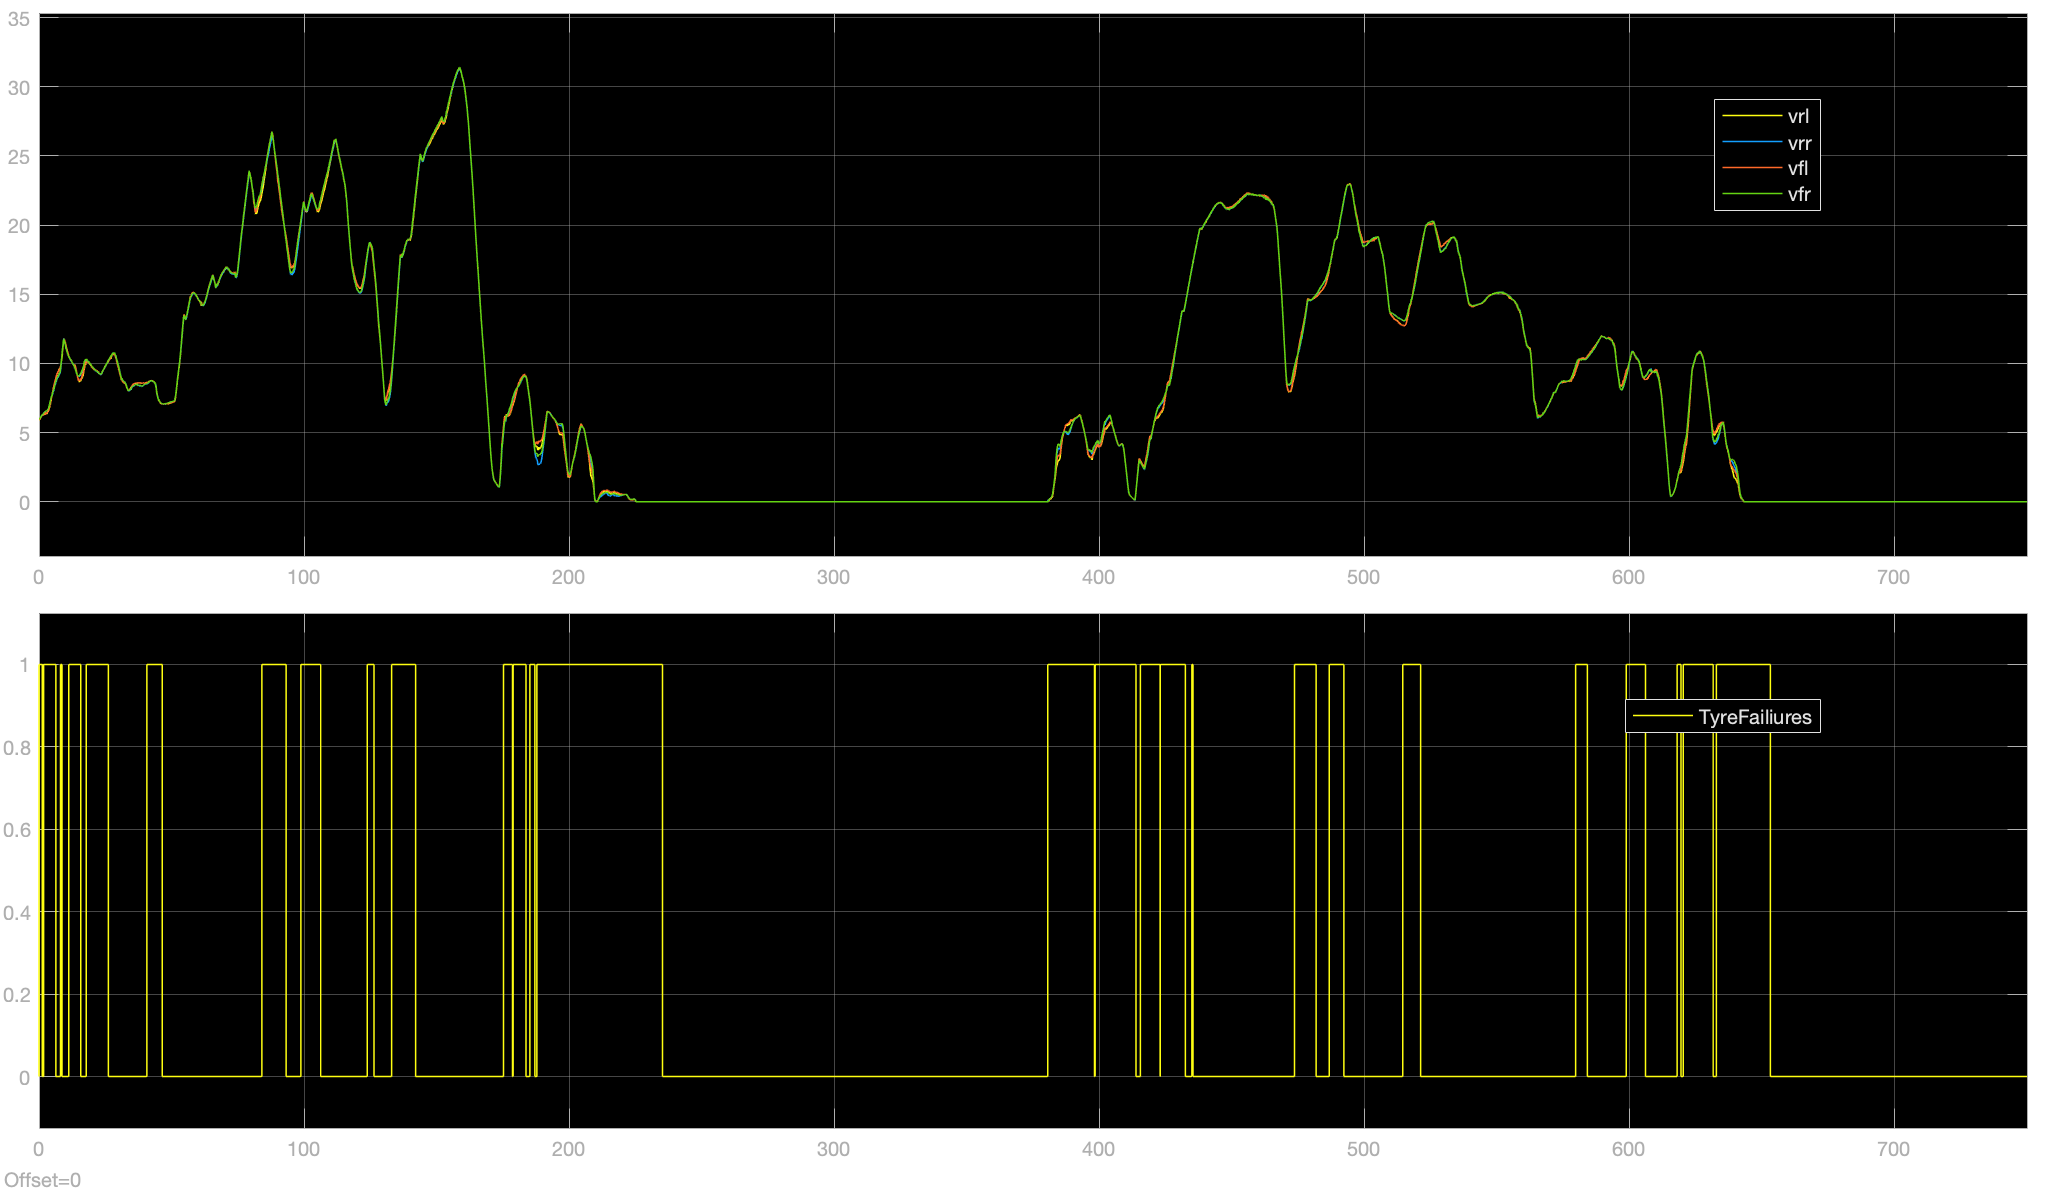
\includegraphics[width=0.95\linewidth]{../Graphiken/CurvesTireMonitor.png}
	\caption{Tire Monitor für Kurvenfahrt}
\end{figure}
Ein Wert von 1  entspricht einer Beobachtung einer Imbalance und ein Wert von 0 entspricht keiner Anomalie.








	
	

	
	
	
	